% !TeX root = RJwrapper.tex
\title{Inequality: Inequality Measurement, Decomposition, and Poverty Analysis in R}


\author{by Charles Coverdale}

\maketitle

\abstract{%
The inequality package provides tools for measuring income and wealth inequality, decomposing it into between-group and within-group components, and relating it to poverty and fiscal redistribution. It covers the Gini coefficient with Davidson (2009) bootstrap and asymptotic confidence intervals, the extended S-Gini family, the generalised entropy family (Theil T and L), the Atkinson and Kolm indices, the Palma ratio, the Hoover index, percentile ratios, Lorenz curves, Bourguignon (1979) between-within decomposition, concentration indices with Erreygers (2009) correction, Kakwani tax progressivity, Reynolds-Smolensky redistribution, Foster-Greer-Thorbecke poverty measures, the Sen and Watts indices, Ravallion-Chen (2003) growth incidence curves, and Wolfson polarisation. Every function accepts optional survey weights. The package is pure R, has no network dependency, and will be available on CRAN shortly.
}

\section{Introduction}\label{introduction}

The \pkg{inequality} package is a comprehensive R implementation of
the indices, decompositions, poverty measures, and redistribution
diagnostics used in applied distributional economics. It accepts raw
income, wealth, or expenditure data from any source, applies optional
survey weights, and returns S3 objects with print methods and cited
underlying references. Eighteen exported functions share a uniform
\code{iq\_} prefix and consistent argument ordering, so a user who
knows \code{iq\_gini()} can reach for \code{iq\_atkinson()},
\code{iq\_theil()}, or \code{iq\_kakwani()} without re-reading
documentation.

The state of R infrastructure for inequality measurement is poor
relative to the demand. The main package on CRAN, \CRANpkg{ineq}, was
last updated in 2014. It computes the Gini and Theil indices and
renders a Lorenz curve, but it has no support for survey weights,
no confidence intervals, no between-within decomposition, no poverty
measures, no Palma ratio, no tax progressivity, and no concentration
indices. Distributional analysis of contemporary survey data, from the
Luxembourg Income Study to the UK Family Resources Survey to the
Australian Household Income and Labour Dynamics survey, requires all
of these as routine operations. Researchers have worked around the
gap with ad hoc code that is neither tested nor cited;
\pkg{inequality} consolidates the operations they actually need
behind a single consistent interface.

The package is pure computation, with four runtime imports
(\CRANpkg{cli}, \code{grDevices}, \code{graphics}, \code{stats}),
three of which ship with base R. There are no API calls, no network
access, and no bundled upstream data. Every numerical result is
reproducible given the input; the only source of randomness is the
Gini bootstrap confidence interval, which exposes a seed-controllable
argument.

\section{Background}\label{background}

Inequality measurement has accumulated four broad families of indices
over the past century.

\textbf{Rank-based indices.} The Gini coefficient \citep{gini1912variabilita}
averages the absolute difference in income between all pairs of
individuals, normalised by twice the mean. Geometrically it is twice
the area between the Lorenz curve \citep{lorenz1905methods} and the line of
perfect equality. The Gini is scale-invariant and transfer-sensitive
but anonymous with respect to distributional position: a transfer from
rich to poor and from middle to middle contribute equally when they
span the same percentile gap. The S-Gini family
\citep{donaldson1980single} adds a parameter that reweights transfers by
rank.

\textbf{Axiomatic indices.} Theil T and L \citep{theil1967information},
generalised by \citet{shorrocks1980class} into the generalised entropy (GE)
family indexed by \(\alpha\), admit additive between-within
decomposition (an axiom the Gini does not satisfy in general). The
Atkinson index \citep{atkinson1970measurement} is grounded in social
welfare: its parameter \(\varepsilon\) encodes inequality aversion, and
the index equals the fraction of mean income the society would
sacrifice to eliminate inequality while maintaining social welfare.

\textbf{Tail-sensitive ratios.} The Palma ratio \citep{palma2011homogeneous}
compares the income share of the top 10 per cent with that of the
bottom 40 per cent. Percentile ratios such as P90/P10 and P80/P20 are
similar in spirit. These measures are not transfer-sensitive inside
the middle of the distribution by construction, which is a feature
when the analyst cares about tails.

\textbf{Absolute indices.} Scale-invariance is appropriate for
cross-country comparisons but not for assessing whether an individual
economy's inequality is rising. The Kolm index
\citep{kolm1976unequal} is translation-invariant instead: it is unchanged
by equal absolute additions to every income. The Hoover index
measures the share of total income that would need to be redistributed
to achieve perfect equality.

\textbf{Decomposition.} \citet{bourguignon1979decomposable} shows that the GE
family is the unique class of scale-invariant indices admitting exact
additive decomposition into between-group and within-group components.
This result is the reason distributional economists routinely
decompose inequality into that attributable to covariates (education,
region, gender) and that within each stratum.

\textbf{Poverty.} The Foster-Greer-Thorbecke family
\citep{foster1984class} parameterises headcount, gap, and severity by
\(\alpha\). The Sen index \citep{sen1976poverty} combines headcount,
poverty gap, and Gini of the poor into a single measure that
satisfies the monotonicity and transfer axioms. The Watts index is an
early axiomatic alternative. \citet{ravallion2003measuring} introduced the
growth incidence curve, which plots the annualised growth rate of
real income at each percentile, turning the question ``was growth
pro-poor?'' into a directly-visible curve.

\textbf{Fiscal redistribution.} \citet{kakwani1977measurement} defines tax
progressivity as the concentration index of taxes paid minus the Gini
of pre-tax income. \citet{reynolds1977public} show that the difference
between pre-tax and post-tax Gini decomposes cleanly into Kakwani
progressivity times average tax rate, plus a reranking term. These
diagnostics are central to distributional fiscal incidence analysis.

\textbf{Polarisation.} \citet{foster2010polarization} argue that inequality and
bipolarisation are conceptually distinct: the same Gini is consistent
with a unimodal distribution and with a bimodal ``disappearing middle''
distribution. The Wolfson polarisation index, developed further in
that paper, is designed to separate the two.

\textbf{Concentration and health.} The concentration index, related to the
Gini but computed against a ranking variable (usually income) rather
than the measured variable (usually health), quantifies socioeconomic
gradients in health outcomes. \citet{erreygers2009correcting} proposes a
correction that restores symmetry in ill-being versus well-being
framings.

\section{Package design}\label{package-design}

\pkg{inequality} is pure R with no compiled code. Runtime imports
are \CRANpkg{cli} (user-facing messages and errors), \code{grDevices},
\code{graphics}, and \code{stats}. R 4.1.0 or later is required. The
only suggested package is \CRANpkg{testthat} for the test suite. The
package has no API clients, no bundled external data (beyond a
synthetic data generator), and no optional heavy dependencies.

Every exported function is prefixed \code{iq\_} and takes a numeric
vector of incomes, wealth, or outcomes as its first argument, followed
by an optional \code{weights} vector and an \code{na.rm} flag.
Index-specific parameters follow: \code{epsilon} for
\code{iq\_atkinson()}, \code{index} (for choosing T or L) for
\code{iq\_theil()} and \code{iq\_decompose()}, \code{line} for
\code{iq\_poverty()}. The return is always an S3 object with a
\code{print()} method; the list elements can be extracted with the
familiar \code{\$} accessor.

Every index and diagnostic accepts a \code{weights} argument
corresponding to survey sampling weights or frequency weights.
Weighted quantiles use the Hyndman-Fan Type 7 linear interpolation,
matching \code{stats::quantile()} defaults. Weighted mean and variance
use the standard formulae. This parity matters: survey data is the
dominant input to real-world inequality analysis, and the legacy CRAN
package \CRANpkg{ineq} requires the user to expand the survey into a
row-per-person data frame before computing any index, which is
memory-prohibitive for anything beyond toy samples.

The Gini coefficient admits two inferential routes. The asymptotic
variance, derived in \citet{davidson2009reliable}, is computed from a single
pass over the data. The bootstrap route resamples the data
\code{R} times (default 1000) and takes percentile-method intervals.
The asymptotic estimator is cheap and accurate in large samples; the
bootstrap is slower but behaves better under heavy-tailed income
distributions where the asymptotic distribution can be slow to
settle. Both are selected via \code{method = "asymptotic"} or
\code{method = "bootstrap"} to \code{iq\_gini(..., ci = TRUE)}.

Each family of functions has its own S3 class. Inequality indices
return \code{iq\_gini}, \code{iq\_atkinson}, and \code{iq\_theil}
objects. Distribution and decomposition functions return
\code{iq\_lorenz} and \code{iq\_decomposition}. Poverty and growth
functions return \code{iq\_poverty} and \code{iq\_growth\_incidence}.
Utility functions return \code{iq\_comparison} or
\code{iq\_concentration}. All classes expose a \code{print()}
method emitting a compact summary. \code{plot()} methods are
provided for \code{iq\_lorenz} and for
\code{iq\_growth\_incidence}, where geometric intuition matters.

Numerical results are deterministic given the input. The only random
component is the bootstrap in \code{iq\_gini()} and
\code{iq\_compare()}, which accepts a \code{seed} argument for exact
reproducibility. The package ships a synthetic data generator,
\code{iq\_sample\_data()}, that produces income, panel, and grouped
data frames with a fixed seed, used in examples and in the canonical
replication below.

\section{Inequality indices}\label{inequality-indices}

\code{iq\_gini(x, weights, ci, method, R, level)} returns the Gini
coefficient with optional confidence intervals. Figure
\ref{fig:lorenz} shows the Lorenz curves of three distributions with
Gini 0.20, 0.43, and 0.69; by construction the curves are nested, and
the area between each curve and the 45-degree line is half the Gini.

\begin{figure}[H]

{\centering 
\includegraphics[width=1\linewidth,alt={A chart showing three Lorenz curves nested between the origin and the top-right corner of a square, alongside a dashed diagonal representing perfect equality. The innermost curve, close to the diagonal, corresponds to a Gini of 0.20; the middle curve to a Gini of 0.43; the outermost curve, furthest from the diagonal, to a Gini of 0.69. All three curves are monotonic and convex.},]{figures/fig1_lorenz} 

}

\caption{Lorenz curves for three synthetic income distributions with low, medium, and high inequality. Each series is a lognormal sample of 2000 observations. Distributions share the same geometric mean and differ only in dispersion. Dashed diagonal is the line of perfect equality. Each Gini is twice the area between its curve and the diagonal.}\label{fig:lorenz}
\end{figure}

Figure \ref{fig:gini-ci} shows how the Davidson bootstrap confidence
interval width shrinks with sample size. At 100 observations the
half-width is over 0.05 Gini points, which is often larger than the
substantive effect an applied economist is trying to detect. At 5000
observations the interval collapses to under 0.02 Gini points.

\begin{figure}[H]

{\centering 
\includegraphics[width=1\linewidth,alt={A chart of confidence interval half-width on the vertical axis against sample size on a logarithmic horizontal axis. Values fall from above 0.05 at a sample size of 100 to below 0.02 at a sample size of 5000. The curve is smoothly decreasing and approximately linear in log space.},]{figures/fig2_gini_ci} 

}

\caption{Mean 95 per cent Davidson bootstrap CI width for the Gini coefficient as a function of sample size. At each sample size the CI is computed on 40 independent lognormal draws (mu = 10.5, sigma = 0.8), each with 400 bootstrap replications. Sample sizes on the log scale. CI half-width falls by a factor of roughly six between n = 100 and n = 5000.}\label{fig:gini-ci}
\end{figure}

\code{iq\_theil()} returns either Theil T (GE(1)) or Theil L
(GE(0)) depending on the \code{index} argument.
\code{iq\_atkinson()} returns the Atkinson index with its
equally-distributed-equivalent income. The remaining inequality
measures are exposed through \code{iq\_kolm()},
\code{iq\_palma()}, \code{iq\_hoover()}, \code{iq\_sgini()}, and
\code{iq\_percentile\_ratio()} complete the set of inequality
indices.

\section{Decomposition and income shares}\label{decomposition-and-income-shares}

\code{iq\_decompose(x, group, weights, index)} implements the
Bourguignon decomposition of a GE index into a between-group
component (the inequality that would remain if every individual had
their group mean) and a within-group component (the inequality that
would remain if every group had the grand mean). Figure
\ref{fig:decompose} shows how the decomposition behaves across three
grouping scenarios, holding within-group dispersion constant but
varying the spread of group means.

\begin{figure}[H]

{\centering 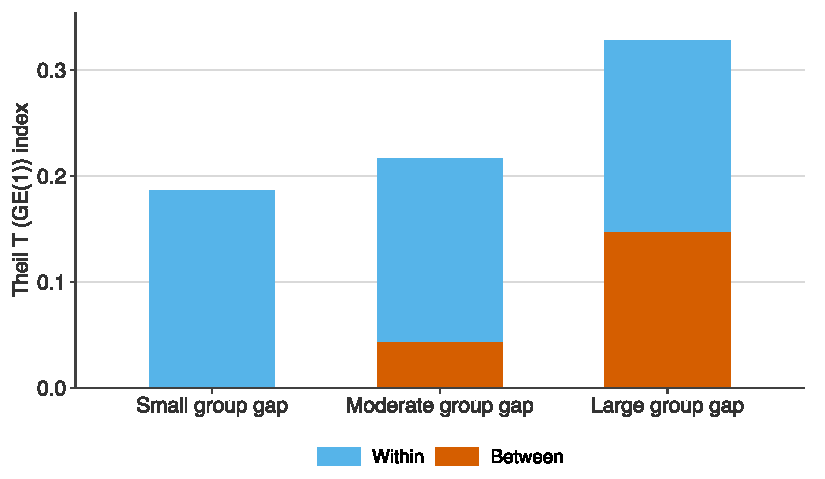
\includegraphics[width=1\linewidth,alt={A stacked bar chart with three bars, each representing a different grouping scenario. Every bar is normalised to the same total height, representing the full Theil T index. The left bar is dominated by the within-group component (the between share is 0.6 per cent). The middle bar has a larger between-group share. The right bar is roughly evenly split, with the between-group share reaching 45 per cent.},]{figures/fig3_decompose} 

}

\caption{Bourguignon between-within decomposition of Theil T across three grouping scenarios. Each scenario has 1500 observations in three groups with identical within-group dispersion (sigma = 0.6 lognormal) but different group-mean spread. Left bar: group means GBP 30k / 32k / 34k, between share 0.6 per cent. Middle bar: group means 25k / 35k / 55k. Right bar: group means 18k / 40k / 80k, between share 45 per cent. The between-within split is an immediate diagnostic for how much inequality is explained by the grouping variable.}\label{fig:decompose}
\end{figure}

\code{iq\_shares(x, weights)} returns the income share held by the
bottom 50 per cent, the middle 40 per cent, the top 10 per cent, and
the top 1 per cent. This mirrors the tabulation style of the World
Inequality Database and Distributional National Accounts.

\code{iq\_concentration()} computes the concentration index of a
health or wellbeing variable against a rank variable (usually
income). The \code{corrected = TRUE} option applies the Erreygers
correction for bounded variables.

\code{iq\_lorenz()} returns the Lorenz curve coordinates and the
associated Gini. A \code{plot()} method renders the curve with
the line of perfect equality.

\section{Poverty and growth incidence}\label{poverty-and-growth-incidence}

\code{iq\_poverty(x, line, weights, alpha)} returns the FGT headcount
(\(\alpha = 0\), the poverty rate), gap (\(\alpha = 1\), depth of poverty
normalised by the line), and severity (\(\alpha = 2\), which rewards
transfers within the poor), plus the Sen index and the Watts index.
The poverty line is a required argument with no default, since the
choice of line is a substantive modelling decision.

\code{iq\_growth\_incidence(x\_t0, x\_t1, weights, n\_quantiles)}

returns the Ravallion-Chen growth incidence curve, plotting
annualised income growth at each percentile of the period-zero
distribution. The mean growth rate corresponds to the usual
aggregate growth statistic; a curve below the mean line at low
percentiles indicates anti-poor growth. Figure \ref{fig:gic} shows a
curve from the package's sample panel dataset.

\begin{figure}[H]

{\centering 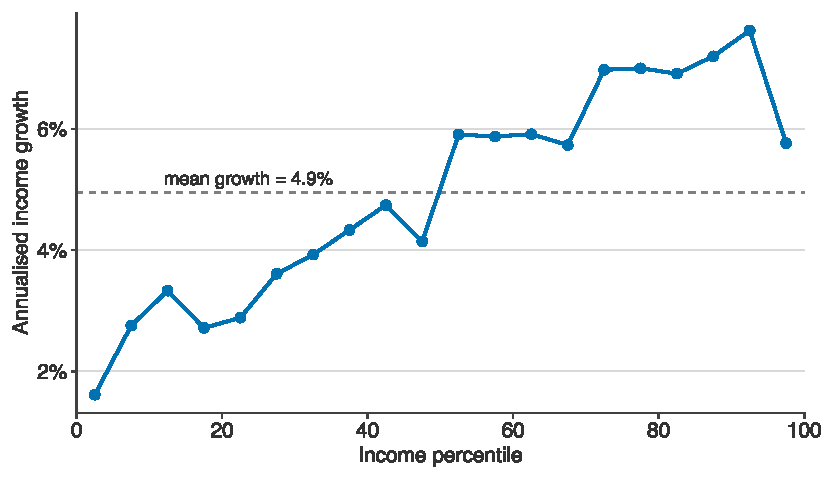
\includegraphics[width=1\linewidth,alt={A line chart with the base-period percentile rank on the horizontal axis from 0 to 100 and the annualised growth rate on the vertical axis. The curve rises monotonically from a low value at the lowest percentile to a higher value at the top percentile. A horizontal dashed line marks the mean annualised growth rate; the curve is below the dashed line for lower percentiles and above it at higher percentiles.},]{figures/fig4_gic} 

}

\caption{Growth incidence curve on the package's synthetic panel dataset. Data from \texttt{iq\_sample\_data("panel")}: 1000 individuals across two periods, lognormal returns with heterogeneous growth (lower percentiles grow more slowly). Annualised growth rate at each 5-percentile bin is plotted against the base-period percentile rank. Dashed line is the mean annualised growth rate across the full distribution. The curve's upward slope signals inequality-increasing growth over the period.}\label{fig:gic}
\end{figure}

\section{Fiscal redistribution and polarisation}\label{fiscal-redistribution-and-polarisation}

\code{iq\_kakwani(pre\_tax, tax, weights)} returns the Kakwani index
of tax progressivity (concentration index of the tax minus Gini of
pre-tax income) and the Reynolds-Smolensky index of redistribution
(Gini of pre-tax income minus Gini of post-tax income). By
construction redistribution decomposes into progressivity times
average tax rate less a reranking term.

\code{iq\_polarisation(x, weights)} returns the Wolfson polarisation
index. The index is zero under perfect equality, reaches a positive
maximum when the distribution splits into two equal masses far from
the median, and is uncorrelated with the Gini in general. Rising
polarisation with stable Gini is the empirical signature of a
``disappearing middle''.

\section{A case study on the inequality verdict}\label{a-case-study-on-the-inequality-verdict}

A common pitfall in distributional analysis is treating a single
index as synonymous with ``inequality''. Different indices weight
different parts of the distribution, so the ordinal ranking of two
populations can flip depending on the index chosen. Figure
\ref{fig:atkinson} makes this concrete: two distributions are scored
by the Atkinson index over a grid of inequality-aversion parameters
\(\varepsilon \in [0.1, 2.5]\). A lognormal distribution scores
consistently lower than a heavy-tailed mixture (85 per cent
moderate-variance plus 15 per cent high-variance top tail) throughout
the range, but the gap between them widens sharply with
\(\varepsilon\): the heavy-tailed distribution is penalised far more
once the social welfare function becomes aversive to inequality at
the top.

\begin{figure}[H]

{\centering 
\includegraphics[width=1\linewidth,alt={A line chart with the inequality-aversion parameter epsilon on the horizontal axis from 0.1 to 2.5 and the Atkinson index value on the vertical axis. A solid blue line corresponds to a lognormal sample and rises gently. A dashed red line corresponds to a heavy-tailed mixture and rises much more steeply, reaching roughly double the blue line by epsilon equals 2.},]{figures/fig5_atkinson} 

}

\caption{Atkinson index as a function of inequality-aversion parameter epsilon for two distributions. Blue solid: a single lognormal sample, n = 3000. Red dashed: a mixture, 85 per cent moderate lognormal plus 15 per cent high-mean high-variance lognormal, total n = 3000. At epsilon = 0.5 the two distributions score similarly; at epsilon = 2 the mixture distribution scores more than double the lognormal, reflecting the heavier top tail. The two distributions have Gini coefficients 0.41 and 0.56 respectively.}\label{fig:atkinson}
\end{figure}

The practical implication is that any claim of the form ``population A
is more unequal than population B'' requires specifying the index. The
\code{iq\_compare()} function addresses this by running the standard
index set on the same data and returning the tabulated results.

\section{A case study of six-country inequality trajectories}\label{a-case-study-of-six-country-inequality-trajectories}

Figure \ref{fig:wb-gini} plots annual Gini coefficients from the
World Bank's Poverty and Inequality Platform (PIP), series
\code{SI.POV.GINI}, for six economies with the longest continuous
coverage: Sweden, Germany, France, the United Kingdom, the United
States, and Brazil, 1970 to 2024. The Gini values themselves are
published; the case study's contribution is to show how the package
machinery handles the full observed record (241 country-year
observations) in one pipeline and to produce a Davidson-interval
point estimate on any slice the user cares about.

\begin{figure}[H]

{\centering 
\includegraphics[width=1\linewidth,alt={A line chart with calendar year on the horizontal axis from 1970 to 2024 and Gini coefficient on the vertical axis from about 22 to 60. Six country series are plotted. Brazil sits well above the others, starting around 58 and declining to about 50. The United States climbs from 37 to 42. Sweden, France, and Germany cluster between 25 and 33 across the full period. The United Kingdom rises from 28 to 32 with most of the increase in the 1980s.},]{figures/fig6_wb_gini} 

}

\caption{Gini coefficient by country, 1970 to 2024, from the World Bank Poverty and Inequality Platform. Data: World Bank series \texttt{SI.POV.GINI}, downloaded via the WDI API. Six economies with the longest continuous coverage are shown. Brazil shows the well-documented post-Bolsa-Familia decline from 58 in 1989 to 51 in 2024. The United States shows a steady rise from 37 in 1970 to 42 in 2024. Sweden, France, Germany cluster in the 25 to 32 band throughout. The United Kingdom traces a Thatcher-era rise and post-1990 stabilisation.}\label{fig:wb-gini}
\end{figure}

Table \ref{tab:wb-summary} reports the first-year and last-year
Gini and the point change for each country.

\begin{table}[H]
\centering
\caption{\label{tab:wb-summary}First-year and last-year Gini plus total change for six countries in the World Bank Poverty and Inequality Platform panel. Ordered by latest observed Gini, ascending. Change is the last-year Gini minus the first-year Gini in percentage points.}
\centering
\begin{tabular}[t]{lrrrrl}
\toprule
Country & First & First Gini & Last & Last Gini & Change (pp)\\
\midrule
Sweden & 1975 & 24.3 & 2023 & 29.3 & +5.0\\
France & 1970 & 37.1 & 2023 & 31.8 & -5.3\\
United Kingdom & 1970 & 28.0 & 2021 & 32.4 & +4.4\\
Germany & 1991 & 29.3 & 2022 & 33.7 & +4.4\\
United States & 1970 & 36.6 & 2024 & 41.8 & +5.2\\
\addlinespace
Brazil & 1981 & 57.9 & 2024 & 50.3 & -7.6\\
\bottomrule
\end{tabular}
\end{table}

The picture is consistent with the comparative-welfare literature
\citep{atkinson2008changing, piketty2014capital}: Scandinavian
economies with strong redistribution remain at the low end of the
distribution; liberal-market economies (United States, United
Kingdom) saw rising inequality from roughly 1980; continental
European economies traced a middle path; and Brazil's post-2000
declines track the expansion of conditional-cash-transfer
programmes.

The computation itself is two lines: read the CSV, pass each
country's series to \code{iq\_gini()} to obtain a Davidson bootstrap
confidence interval if desired. The bundled \pkg{inequality}
toolkit then allows any of the other indices (Theil, Atkinson,
Palma) to be computed from the same underlying microdata when
available, and the between-within decomposition described above to
treat the country as the grouping variable for a cross-country
decomposition of global inequality.

\section{Replication}\label{replication}

Table \ref{tab:compare} reports \code{iq\_compare()} output on the
package's synthetic sample data. The data frame has 1000 observations
drawn from a lognormal distribution with mean log 10.5 and standard
deviation log 0.8; the sample is bundled via
\code{iq\_sample\_data("income")}.

\begin{table}[H]
\centering
\caption{\label{tab:compare}Nine inequality and poverty indices for the package's synthetic income sample. Output of \texttt{iq\_compare(iq\_sample\_data("income")\$income)}. Gini and Theil agree on the total magnitude; Atkinson rises sharply with inequality aversion; Palma ratio captures the 10/40 tail concentration; P90/P10 gives the most intuitive read.}
\centering
\begin{tabular}[t]{lr}
\toprule
Index & Value\\
\midrule
Gini & 0.4300\\
Theil T (GE1) & 0.3307\\
Theil L (GE0) & 0.3241\\
Atkinson (e=0.5) & 0.1506\\
Atkinson (e=1.0) & 0.2768\\
\addlinespace
Palma ratio & 2.1528\\
Hoover & 0.3126\\
P90/P10 & 7.8282\\
P80/P20 & 3.9206\\
\bottomrule
\end{tabular}
\end{table}

The full workflow for an applied study is five lines.

\begin{verbatim}
library(inequality)
d <- iq_sample_data("income")
iq_gini(d$income, weights = d$weight, ci = TRUE)
iq_decompose(d$income, d$group, weights = d$weight)
iq_poverty(d$income, line = 20000, weights = d$weight)
\end{verbatim}

Each call returns an S3 object with a print method; the numeric
components are accessible by \code{\$}.

\section{Limitations}\label{limitations}

Five limitations apply.

\begin{enumerate}
\def\labelenumi{\arabic{enumi}.}
\tightlist
\item
  \pkg{inequality} is a measurement package, not a survey-design
  package. It accepts survey weights but does not compute
  replicate-weight or Taylor-series variance estimators for complex
  survey designs. Users needing design-based inference should pair
  these functions with \CRANpkg{survey} or \CRANpkg{srvyr}.
\item
  The package does not correct for top-coding, bottom-coding, or
  unit non-response. Analyses of administrative tax data are
  sensitive to the top-coding threshold, and the user must apply
  any correction (Pareto tail interpolation, for example) before
  passing data into the functions.
\item
  Inferential coverage is confined to the Gini coefficient.
  Confidence intervals for the other indices could be added by
  bootstrap but are not yet exposed as a uniform option.
\item
  The package does not reconcile survey income to national accounts,
  as the Distributional National Accounts (DINA) framework does.
  Cross-comparability of inequality indices across countries and
  vintages remains the user's responsibility.
\item
  All functions are pure R. For panel inequality analysis at the
  scale of linked employer-employee data (millions of rows across
  dozens of time periods), compiled-code implementations in Rcpp or
  Julia would be faster.
\end{enumerate}

\section{Conclusion}\label{conclusion}

Inequality measurement is mature as a subfield but has been
underserved on CRAN: \CRANpkg{ineq} has not been updated in over a
decade, and applied work has relied on private scripts that are
neither tested nor cited. \pkg{inequality} replaces that state
with a single package that covers every index, decomposition,
poverty measure, and fiscal-redistribution diagnostic routinely used
in applied distributional analysis. All functions accept survey
weights, return cited S3 objects with print methods, and share a
uniform interface. Planned additions for future releases include
complex-survey variance estimators, DINA-style national-accounts
reconciliation helpers, bootstrap confidence intervals for the full
index set, and compiled-code implementations for large panels.
Contributions and bug reports are welcome at
\url{https://github.com/charlescoverdale/inequality}.

\section*{Acknowledgements}\label{acknowledgements}
\addcontentsline{toc}{section}{Acknowledgements}

The author thanks the R Core Team and CRAN maintainers for the
infrastructure that supports open-source statistical software. The
World Bank publishes the Poverty and Inequality Platform series used
in the six-country case study.

\bibliography{RJreferences.bib}

\address{%
Charles Coverdale\\
Independent\\%
London, United Kingdom\\
%
\url{https://github.com/charlescoverdale/inequality}\\%
%
\href{mailto:charles.f.coverdale@gmail.com}{\nolinkurl{charles.f.coverdale@gmail.com}}%
}
